% !TEX root = ../cobar2.tex

%The first map in this composition preserves the coassociative coalgebra structures but not the $\UM$-coalgebra structures.
%Nevertheless, in the following sections, we describe a zig-zag of quasi-isomorphisms of $E_{\infty}$-coalgebras between $\cchains(\ccobarE(X))$ and $\schains(\triangulate\ccobarE(X))$.


\section{\pdfEinfty-structures}

\subsection{Serre--Cartan comparison map}

\anibal{Update this section with new version of cubical paper \cite{medina2022cube_einfty}}

\begin{figure}[h!]
	\centering
	\documentclass{standalone}
\usepackage{tikz}
\usepackage{amsmath}

\begin{document}
	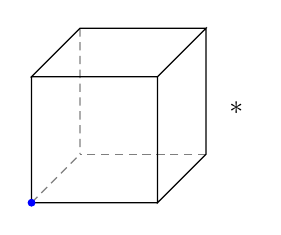
\begin{tikzpicture}[every edge quotes/.append style={auto, text=black}, scale=.4]
		\pgfmathsetmacro{\cubex}{4}
		\pgfmathsetmacro{\cubey}{4}
		\pgfmathsetmacro{\cubez}{4}
		\draw [draw=black, every edge/.append style={draw=black, densely dashed, opacity=.5}, fill=white]
		(0,0,0) coordinate (o) -- ++(-\cubex,0,0) coordinate (a) -- ++(0,-\cubey,0) coordinate (b) edge coordinate [pos=1] (g) ++(0,0,-\cubez) -- ++(\cubex,0,0) coordinate (c) -- cycle
		(o) -- ++(0,0,-\cubez) coordinate (d) -- ++(0,-\cubey,0) coordinate (e) edge (g) -- (c) -- cycle
		(o) -- (a) -- ++(0,0,-\cubez) coordinate (f) edge (g) -- (d) -- cycle;
		\path [every edge/.append style={draw=black, |-|}];

		\draw [blue,fill] (b) circle [radius=3pt];
		\draw[] node at (2.5,-1){$\ast$};
	\end{tikzpicture}
	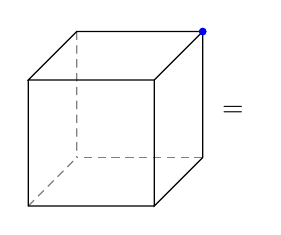
\begin{tikzpicture}[every edge quotes/.append style={auto, text=black}, scale=.4]
		\pgfmathsetmacro{\cubex}{4}
		\pgfmathsetmacro{\cubey}{4}
		\pgfmathsetmacro{\cubez}{4}
		\draw [draw=black, every edge/.append style={draw=black, densely dashed, opacity=.5}, fill=white]
		(0,0,0) coordinate (o) -- ++(-\cubex,0,0) coordinate (a) -- ++(0,-\cubey,0) coordinate (b) edge coordinate [pos=1] (g) ++(0,0,-\cubez) -- ++(\cubex,0,0) coordinate (c) -- cycle
		(o) -- ++(0,0,-\cubez) coordinate (d) -- ++(0,-\cubey,0) coordinate (e) edge (g) -- (c) -- cycle
		(o) -- (a) -- ++(0,0,-\cubez) coordinate (f) edge (g) -- (d) -- cycle;
		\path [every edge/.append style={draw=black, |-|}];

		\draw [blue, fill] (d) circle [radius=3pt];
		\draw[] node at (2.5,-1){$=$};
	\end{tikzpicture}
	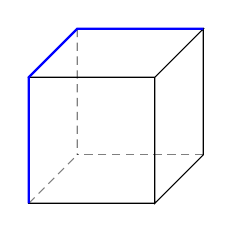
\begin{tikzpicture}[every edge quotes/.append style={auto, text=black}, scale=.4]
		\pgfmathsetmacro{\cubex}{4}
		\pgfmathsetmacro{\cubey}{4}
		\pgfmathsetmacro{\cubez}{4}
		\draw [draw=black, every edge/.append style={draw=black, densely dashed, opacity=.5}, fill=white]
		(0,0,0) coordinate (o) -- ++(-\cubex,0,0) coordinate (a) -- ++(0,-\cubey,0) coordinate (b) edge coordinate [pos=1] (g) ++(0,0,-\cubez) -- ++(\cubex,0,0) coordinate (c) -- cycle
		(o) -- ++(0,0,-\cubez) coordinate (d) -- ++(0,-\cubey,0) coordinate (e) edge (g) -- (c) -- cycle
		(o) -- (a) -- ++(0,0,-\cubez) coordinate (f) edge (g) -- (d) -- cycle;
		\path [every edge/.append style={draw=black, |-|}];

		\draw[blue, thick] (b)--(a)--(f)--(d);
	\end{tikzpicture}
\end{document}
	\caption{Geometric representation of $\big([0]\ot[0]\ot[0] \ast [1]\ot[1]\ot[1]\big)$ where we are using the width-depth-height order.}
	\label{f:product}
\end{figure}

We review from \cite{medina2022cube_einfty} the relationship between the $E_\infty$-structures defined on simplicial chains in \cref{ss:e-infty on simplicial} and on cubical chains in \cref{ss:e-infty on cubical}.

In \cite[p.442]{serre1951homologie}, the \textit{Serre--Cartan collapse} $\gcube^n \to \gsimplex^n$ was introduced and used to define a natural quasi-isomorphism of coalgebras $\sSchains(Z) \to \cSchains(Z)$ for any topological space $Z$.
This map factors as the composition
\[
\schains(\sSing(Z)) \xra{\cartanserre_{\sSing(Z)}}
\cchains(\mathcal{U} \sSing(Z)) \to
\cchains(\cSing(Z)),
\]
where the first map $\cartanserre_X$, referred to as the \textit{Serre--Cartan comparison map}, is a quasi-isomorphism defined for any simplicial set $X$, and the second map is induced from a morphism of cubical sets.

Although both $\schains(X)$ and $\cchains(\mathcal{U} X)$ have natural $\UM$-structures, the map $\cartanserre_X$ is not a morphism of $\UM$-coalgebras for a generic simplicial set $X$.
Nevertheless, after restriction of their $\UM$-structures via an inclusion of $E_\infty$-operads $\USL \to \UM$, the Cartan-Serre comparison map becomes a morphism of $E_\infty$-coalgebras.
The operad $\USL$ is generated as a suboperad of $\UM$ by all immerse connected graphs of the form
\begin{equation*}
\begin{tikzpicture}[scale=1]
\draw (0,0)--(0,-.6) node[below, scale=.75]{$1$};
\draw (0,0)--(.5,.5);
\draw (-.3, .3)-- (-.2,.5) node[scale=.75] at (-.2,.7) {\qquad $1\, \ \ 2\ \ ...\ \ k_1$};
\draw (-.5,.5)--(0,0);
\node[scale=.75] at (.11,.4){$..$.};

\node[scale=.75] at (1,0){$\cdots$};
\node[scale=.75] at (1,-.9){$\cdots$};

\draw (2,0)--(2,-.68) node[scale=.75, below]{$r$};
\draw (2,0)--(2.5,.5);
\draw (1.7, .3)--(1.8,.5) node[scale=.75] at (1.78,.7) {\qquad $1\, \ \ 2\ \ ...\ \ k_r$};
\draw (1.5,.5)--(2,0);
\node[scale=.75] at (2.11,.4){$..$.};

\draw (1,2.5)--(1,3) node[scale=.75, above]{$1$};
\draw (1,2.5)--(0,2) node[scale=.75, below]{$1$};
\draw (.25,2.125)--(.5,2) node[scale=.75, below]{$2$};
\draw (.5,2.25)--(1,2) node[scale=.75, below]{$3$};
\draw (1,2.5)--(2,2) node[scale=.75, below]{\ \quad $n + r$};
\node[scale=.75] at (1.5,1.75){$\cdots$};

\node[scale=.75] at (1,1.3) {$\vdots$};

\node at (2.85,0){};
\end{tikzpicture}
\end{equation*}
where there are no hidden vertices and the strands are joined so that the associated maps $\{1, \dots, k_j\} \to \{1, \dots, n+k\}$ are order-preserving.
From \cite{medina2022cube_einfty} we have the following.

\begin{proposition} \label{p:simplicialandcubical}
	The suboperad $\USL$ of $\UM$ is an $E_\infty$-operad and the Cartan-Serre comparison map
	\[
	\cartanserre_X \colon \schains(X) \to \cchains(\mathcal U X)
	\]
	is a natural quasi-isomorphism of $\USL$-coalgebras for any simplicial set $X$.
\end{proposition}

We will denote by $\chains_\USL$ the functor of (cubical or simplicial) chains lifted to $\coAlg_\USL$.
We remark that the inclusion $\As \to \UM$ factors through $\USL$ so $\chains_\USL$ is also a lift to a category of $E_\infty$-coalgebras of the functors $\chains_\As$ to $\coAlg$.

\subsection{A zig-zag of \pdfEinfty-coalgebras}
The $E_{\infty}$-coalgebra structures on the simplicial chains on a triangulated cubical set $Y$ and on the cubical chains on $Y$ are related as follows.

\begin{lemma} \label{l:zigzag}
	For any cubical set $Y$ there are natural quasi-isomorphisms of $\USL$-coalgebras
	\begin{equation} \label{e:zig-zag of quasi-isos}
		\schainsUSL(\triangulate Y) \xra{\simeq}
		\cchainsUSL(\mathcal{U}\triangulate Y) \xleftarrow{\simeq}
		\cchainsUSL(Y).
	\end{equation}
\end{lemma}

\begin{proof}
	The first map in \eqref{e:zig-zag of quasi-isos} is a quasi-isomorphism of $\USL$-coalgebras by \cref{p:simplicialandcubical}.
	Whereas the second is induced by the morphism of cubical sets $Y \to \mathcal{U} \triangulate (Y)$ given by the unit of the adjunction
	\[
	\triangulate \colon \cSet \leftrightarrows \sSet :\! \mathcal{U}
	\]
	of \cref{ss:triangulation and its adjoint}.
	The unit map is in fact a weak homotopy equivalence of cubical sets since the adjunction defines a Quillen equivalence between the Kan--Quillen model structure and an analogue model structure on $\cSet$ in which all objects are cofibrant \cite{cisinski2006presheaves}.
	Hence, the unit map induces a quasi-isomorphism of $\USL$-coalgebras after applying the cubical chains functor.
\end{proof}

\subsection{The functor $\adamsE_{\UM}$} \label{s:ahatum}

Define the functor
\[
\adamsEA \colon \sSet^0 \to \Mon_{\coAlg}
\]
as the composition
\[
\adamsEA = \cchainsA \ccobarE.
\]
Similarly define
\[
\adamsE_{\UM} \colon \sSet^0 \to \Mon_{\coAlg_{\UM}}
\]
as the composition
\[
\adamsE_{\UM} = \cchainsUM \ccobarE.
\]

It follows directly from the definitions that $\adamsEA$ is a lift of $\adamsE$, and $\adamsE_{\UM}$ is a lift $\adamsEA$.
This discussion constitutes the first half of \cref{t:2nd main thm in the intro}, which we collect in the following.

\begin{lemma} \label{l:AhatUM}
	The functor $\adamsEUM \colon \sSet^0 \to \Mon_{\coAlg_\UM}$ fits into a commutative diagram
	\[
	\begin{tikzcd}[row sep=small]
		& \Mon_{\coAlg_\UM} \arrow[d] \\
		& \Mon_{\coAlg} \arrow[d] \\
		\sSet^0
		\arrow[r, "\adamsE"', ]
		\arrow[ru, "\adamsEA"', out=45, in=180]
		\arrow[ruu, "\adamsEUM", out=90, in=180]
		& \Mon_{\Ch}.
	\end{tikzcd}
	\]
\end{lemma}


\subsection{The extended cobar construction and the chains on the Kan loop group}

Applying \cref{l:zigzag} to $Y = \ccobarE(X)$, we obtain that $\schainsUSL (\triangulate \ccobarE(X))$ and $\cchainsUSL(\ccobarE(X)) = \adamsE_{\USL}(X)$ are quasi-isomorphic via a zig-zag of natural maps of $\USL$-coalgebras.
By \cref{widehatgcobarandG} we have a weak equivalence of simplicial monoids
\[
\triangulate \ccobarE(X) \xrightarrow{\simeq} \kan(X)
\]
for any reduced simplicial set $X$.
By naturality, we have an induced quasi-isomorphism of $\USL$-coalgebras
\[
\schainsUSL \big( \triangulate \ccobarE(X) \big) \xra{\simeq}
\schainsUSL (\kan(X)).
\]
Therefore, $\adamsE_{\USL}(X)$ and $\schainsUSL(\kan(X))$ are quasi-isomorphic through a zig-zag of natural maps of $\USL$-coalgebras, as desired.
We summarize this discussion in the following lemma, constituting the second half of \cref{t:2nd main thm in the intro}.

\begin{lemma}\label{l:AhatandGX}
	For any reduced simplicial set $X$, there is a zig-zag of natural quasi-isomorphisms of $\USL$-coalgebras between $\adamsE_\USL(X)$ and $\schainsUSL(\kan(X))$.
\end{lemma}